\documentclass[12pt,compress]{beamer}
\usepackage{ifthen,rotating}

\title{Friday September 8 Meeting \\ Minutes (and More)}
\author{Jim Pivarski}
\institute{Texas A\&M University}
\date{13 September, 2006}

\setbeamertemplate{navigation symbols}{}
\setbeamertemplate{headline}{\includegraphics[height=1 cm]{../cmslogo} \hspace{0.1 cm} \includegraphics[height=1 cm]{../tamulogo} \hfill
\begin{minipage}{9 cm}
\vspace{-0.75 cm} \small
\begin{center}
\ifthenelse{\equal{\insertpagenumber}{1}}{}{\insertsection}
\end{center}
\end{minipage} \hfill
\begin{minipage}{1 cm}
\vspace{-0.75 cm} \small
\begin{center}
\ifthenelse{\equal{\insertpagenumber}{1}}{}{\insertpagenumber/\pageref{numpages}}
\end{center}
\end{minipage}}

\xdefinecolor{verylightgray}{rgb}{0.95,0.95,0.95}
\beamertemplateshadingbackground{verylightgray}{white}

\begin{document}
\frame{\titlepage}
\section*{Minutes and More: 8 September --- Jim Pivarski}

\begin{frame}
\frametitle{Available Projects, as we now understand them}
\begin{itemize}
\item ``DetLayers'' and ``MeasurementDet'' are more abstract-coding
projects than physics projects

\item ``Regional track reconstruction'' (\textcolor{blue}{RegionalTrack}) narrowing the
search for {\it silicon} tracks for HLT speed

\item ``Propagation'' (\textcolor{blue}{Propagation}) three algorithms, one is finished
and another is ``almost finished''

\item ``L2MuonReconstruction'' (\textcolor{blue}{L2Seeding}) seeding stand-alone muon
tracks with L1 muon objects for speed in HLT (a slower seeding algo
already exists)
\end{itemize}

\vfill We are interested in \textcolor{blue}{RegionalTrack} or
\textcolor{blue}{L2Seeding} because work is just beginning.  These are
both HLT projects.
\end{frame}

\begin{frame}
\frametitle{RegionalTrack}

\begin{center}
\only<1>{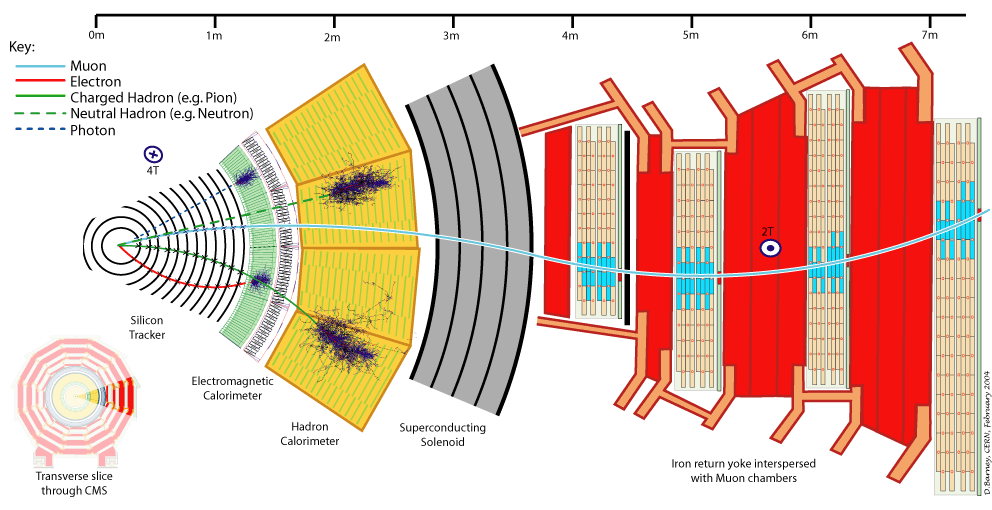
\includegraphics[width=\linewidth]{muon_path}}
\only<2-3>{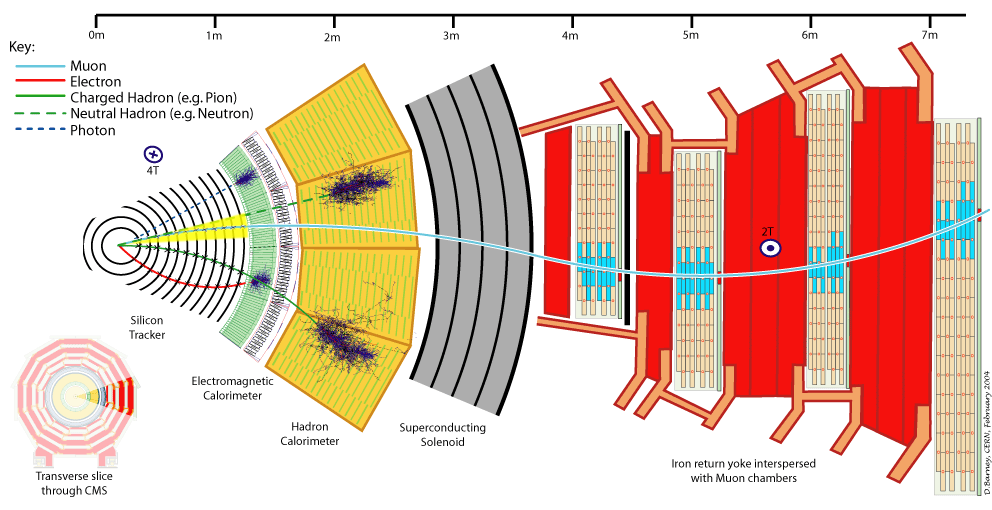
\includegraphics[width=\linewidth]{muon_path2}}

\only<1>{\vfill \begin{tabular}{p{0.45\linewidth} p{0.45\linewidth}}
\begin{minipage}{\linewidth}
\begin{center}
$\delta p_T/p_T$ is 1.0 to 1.5\% for global 10~GeV tracks
\end{center}
\end{minipage} &
\begin{minipage}{\linewidth}
\begin{center}
$\delta p_T/p_T$ is 8 to 15\% for muon-only 10~GeV tracks
\end{center}
\end{minipage}
\end{tabular}}

\only<2>{\vfill \begin{tabular}{p{0.45\linewidth} p{0.45\linewidth}}
\begin{minipage}{\linewidth}
\begin{center}
Road width in silicon is about 20~cm (yellow)
\end{center}
\end{minipage} &
\begin{minipage}{\linewidth}
\begin{center}
``track {\it should} be unique\ldots''
\end{center}
\end{minipage}
\end{tabular}}

\only<3>{\vfill \begin{tabular}{p{\linewidth}}
\begin{minipage}{\linewidth}
Not rejecting spurious muon signals by checking for {\it existence} of
silicon track; we want to reject real, low-momentum muons.
\end{minipage}
\end{tabular}}

\end{center}
\end{frame}

\begin{frame}
\frametitle{RegionalTrack: What this looked like in ECAL}

\begin{center}
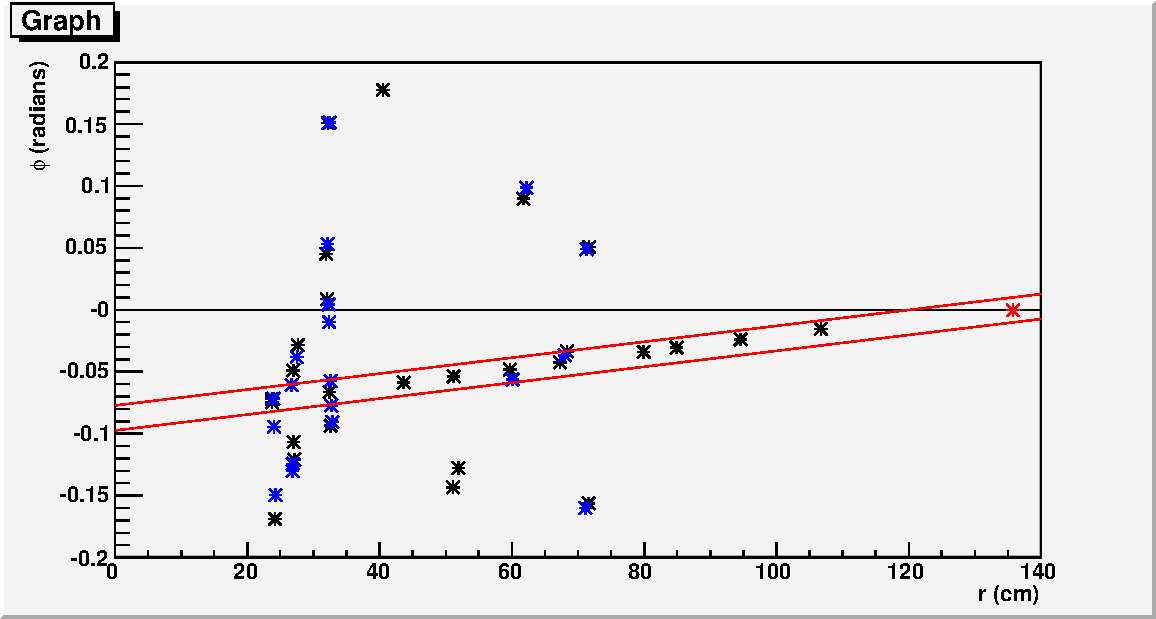
\includegraphics[width=0.7\linewidth]{ecal_event} \hspace{1 cm}\begin{sideways}20 cm = 0.17 rad\end{sideways}
\end{center}
\begin{minipage}{\linewidth}
\small
\begin{itemize}\setlength{\itemsep}{-0.1 cm}
\item Black: rphi silicon-strip hits, Blue: stereo silicon-strip hits
\item Red: ECAL SuperCluster and projection into tracker
\item 10 GeV electron-gun with underlying event (simulated by ONE minbias)
\item vertical axis is $\phi$ position of the HIT, horizontal is radius
\end{itemize}
\end{minipage}
\end{frame}

\begin{frame}
\frametitle{RegionalTrack: What background looked like}

\begin{center}
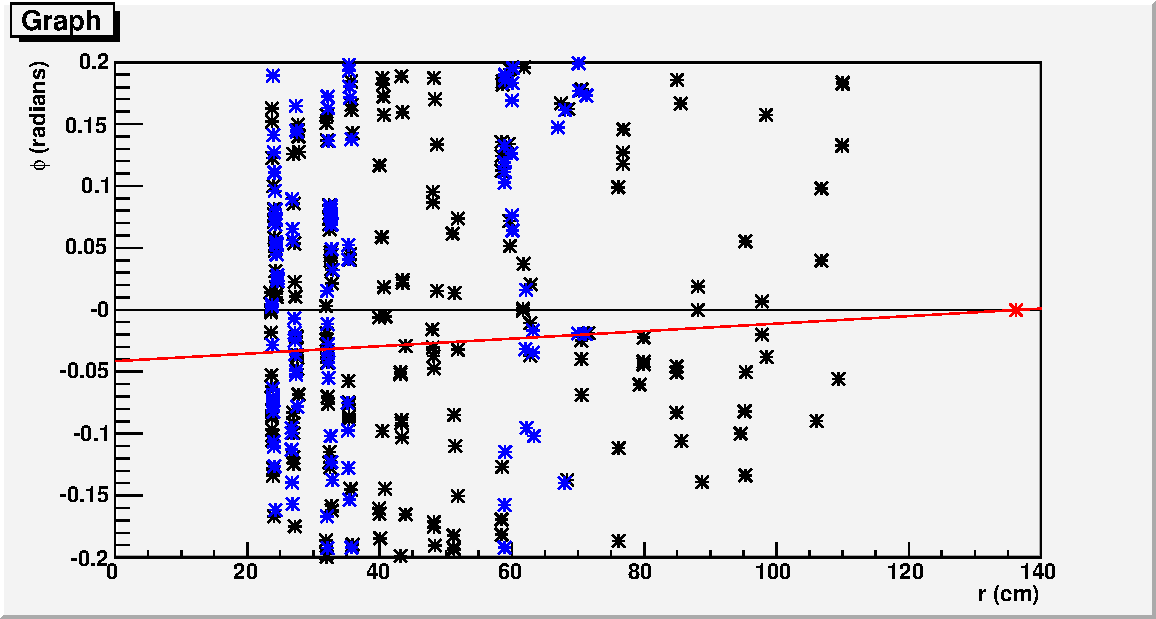
\includegraphics[width=0.7\linewidth]{ecal_background} \hspace{1 cm}\begin{sideways}20 cm = 0.17 rad\end{sideways}
\end{center}
\small
\begin{minipage}{\linewidth}
\begin{itemize}\setlength{\itemsep}{-0.1 cm}
\item Black: rphi silicon-strip hits, Blue: stereo silicon-strip hits
\item Red: ECAL SuperCluster and projection into tracker
\item 20 GeV SuperCluster from a minbias event (jet pointing at calorimeter)
\item vertical axis is $\phi$ position of the HIT, horizontal is radius
\end{itemize}
\end{minipage}
\end{frame}

\begin{frame}
\frametitle{RegionalTrack}

The point is to sharpen resolution for a $p_T$ cut {\it before} doing
full tracking.  Therefore, it must be significantly faster than full
tracking.  It also must cut out enough background:

\begin{quote}
{\bf The non-linear problem} (from ECAL experience): Suppose the
speed and background rejection of an algorithm are inversely related.
The ``slow and thorough'' extreme may be too slow, while ``fast and
dirty'' lets in too much background and may be too slow downstream.
Optimum balance is dictated by physics distributions!
\end{quote}

\vfill \small Jean-Roch Vlimant (postdoc, UCSB) \textless vlimant@fnal.gov\textgreater

Jeff Richman (prof., UCSB) \textless richman@charm.physics.ucsb.edu\textgreater
\end{frame}

\begin{frame}
\frametitle{Propagation}

Three implementations:

\begin{description}\setlength{\itemsep}{0.5 cm}
\item[Slava's SteppingHelixPropagator] completed (send him bug
reports!), fast, hard-coded geometry, hard to update, used now in MTCC

\item[Runge-Kutta] (a.k.a.\ STEP?, ``Navigation geometry propagator''?) almost finished, not debugged

\item[GEANT4] ``is slow.''  We don't know who's working on it.
\end{description}

\vfill
A lot of work has already been done; we'll probably pass.
\end{frame}

\begin{frame}
\frametitle{L2Seeding}

To seed stand-alone muon tracks, we currently throw away Level1 muon
trigger info and work from muon hits

\vfill Issues:
\begin{enumerate}
\item HLT would be faster if we take advantage of Level1 info
\item easier to estimate trigger efficiency if high-level muons
correspond to trigger muons in some way
\end{enumerate}

\vfill All that needs to be done is to write a producer which turns L1
muons into L2 TrackingSeeds?  And then study the performance?

\vfill \small Riccardo Bellan (grad, Universit\'a Degli Studi di Torino) \textless bellan@cern.ch\textgreater

\label{numpages}
\end{frame}

\end{document}
